\chapter{神经网络处理器编译器验证思路}

\begin{figure}[!htbp]
\centering
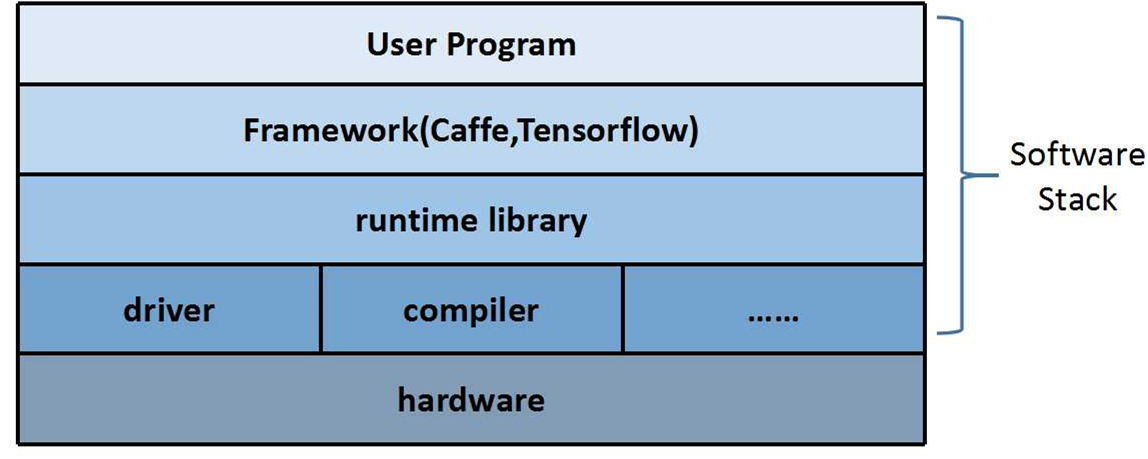
\includegraphics[width=12cm]{Software_stock.jpg}
\caption{神经网络处理器的软件架构}
\label{fig:Software stock}
\end{figure}
\subsection{深度学习指令集的特性}

prototxt -proto-caffe重载,生成随机网络,运行两次caffe 分别获得ipu 结果和cpu 结果,对比结果是否正确,达到验证目的。
\section{protext的生成}

\section{proto的创建}

\section{caffe重载}

\section{caffe运行ipu的过程}
Cpu 准备数据和指令,拷贝到ipu ,ipu 执行,cpu 读结果